\section{Wave}
    \subsection{Simple harmonic motion}
        \paragraph{Defination}
            Simple Harmonic Motion is motion in which net force on an object is propotional to negative of the displacement.
            \begin{align}
                F \propto -x
            \end{align}

        \paragraph{Abstract Model}
            Shown in Figure \ref{shm_md}, the $x$-$t$ relation is a model of simple harmonic motion. The line is rotating with angular speed $\omega$ and initial angle $\phi$. The radius is $x_0$.
            \begin{figure}[H]
                \begin{center}
                    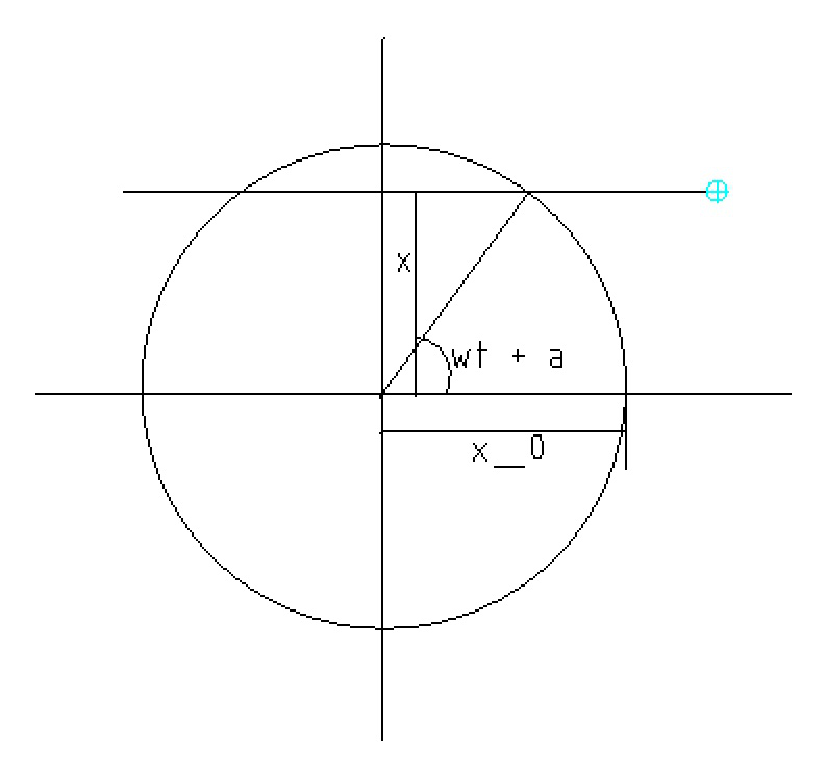
\includegraphics[height=5cm]{wave_charts/shm_circ.eps}
                \end{center}
                \caption{Model of simple harmonic motion}
                \label{shm_md}
            \end{figure}

        
            \begin{align}
                x &= x_0 \sin (\omega t + \phi) \\
                v &= \frac{\mathrm{d} x}{\mathrm{d} t} = x_0 \omega \cos (\omega t + \phi) \\
                a &= \frac{\mathrm{d} v}{\mathrm{d} t} = - x_0 \omega^2 \sin (\omega t + \phi) \\
                  &= - \omega^2 x
            \end{align}

        \paragraph{Spring}
            For an object on a spring, for displacement $x$, the net force act on it is $F = -kx$. Thus, it is SHM.
            \begin{align}
                \left\{
                    \begin{aligned}
                        a &= \frac{F}{m} = \frac{-k x}{m} = - \omega^2 x \\
                        x &= x_0 \sin(\omega t + \phi)
                    \end{aligned}
                \right. & \Rightarrow 
                \frac{-k x}{m} = - \omega^2 x \\
                & \Rightarrow \omega = \sqrt{\frac{k}{m}}
            \end{align}

            \begin{align}
                \therefore T &= \frac{2 \pi}{\omega} \\
                             &= 2 \pi \sqrt{\frac{m}{k}}
            \end{align}

        \paragraph{Pendulum}
            Similarly,
            \begin{align}
                T = 2 \pi \sqrt{\frac{l}{g}}
            \end{align}
            
            Note: only for small angle which $\sin \theta \approx \theta$.

    \subsection{Intensity}
        \paragraph{Properties of wave}
            Wave have following properties:
            \begin{enumerate}
                \item Speed $v$
                \item Period $T$
                \item Amplitude $A$
                \item Wave length $\lambda$
                \item Frequency $f$
            \end{enumerate}

            \begin{figure}[H]
                \begin{center}
                    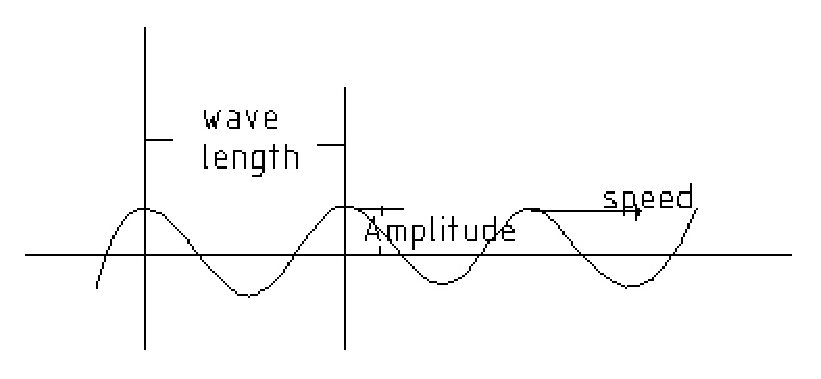
\includegraphics[height=3cm]{wave_charts/wave_prop.eps}
                \end{center}
                \caption{Properties of wave}
                \label{wave_prop}
            \end{figure}

            \begin{align}
                f = \frac{1}{T} = \frac{v}{\lambda}
            \end{align}

        \paragraph{Intensity of wave}
            $\mbox{Intensity} = \frac{\mbox{Power}}{\mbox{Area}}$

            For example, for a wave source with total power $P_0$ radiate to all direction, at distance $r$ from the center, as shwon in Figure \ref{ball_int},
            \begin{figure}[H]
                \begin{center}
                    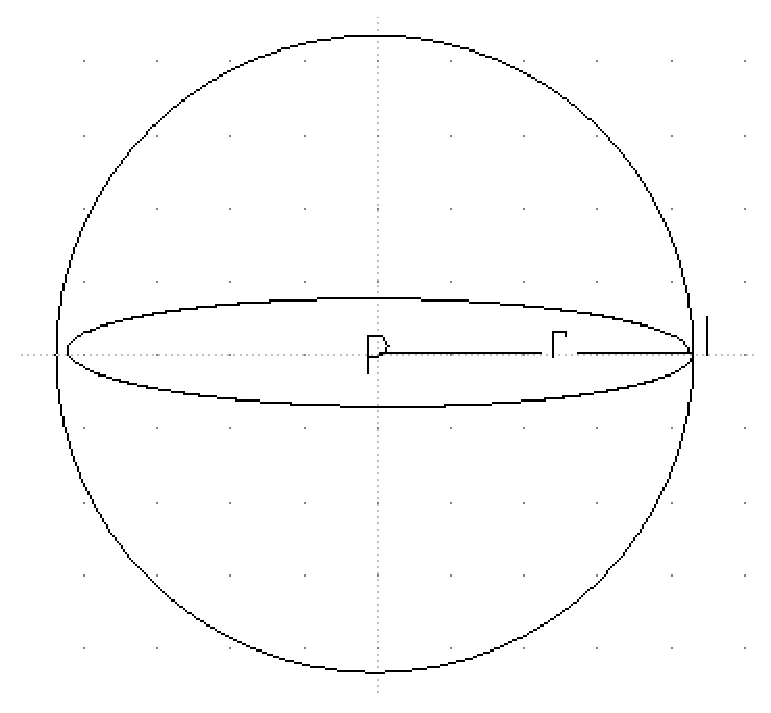
\includegraphics[height=3cm]{wave_charts/ball_intensity.eps}
                \end{center}
                \caption{Intensity at distance $r$}
                \label{ball_int}
            \end{figure}
            
            
            the intensity is

            \begin{align}
                I = \frac{P}{A} = \frac{P_0}{4 \pi r^2}
            \end{align}

    \subsection{Polarization}
        \paragraph{Direction of polarization}
            For polarization grating, as shown in Figure \ref{pol_dir} the polarized wave only with oscillate direction parallel to grating direction can fully pass.

            \begin{figure}[H]
                \begin{center}
                    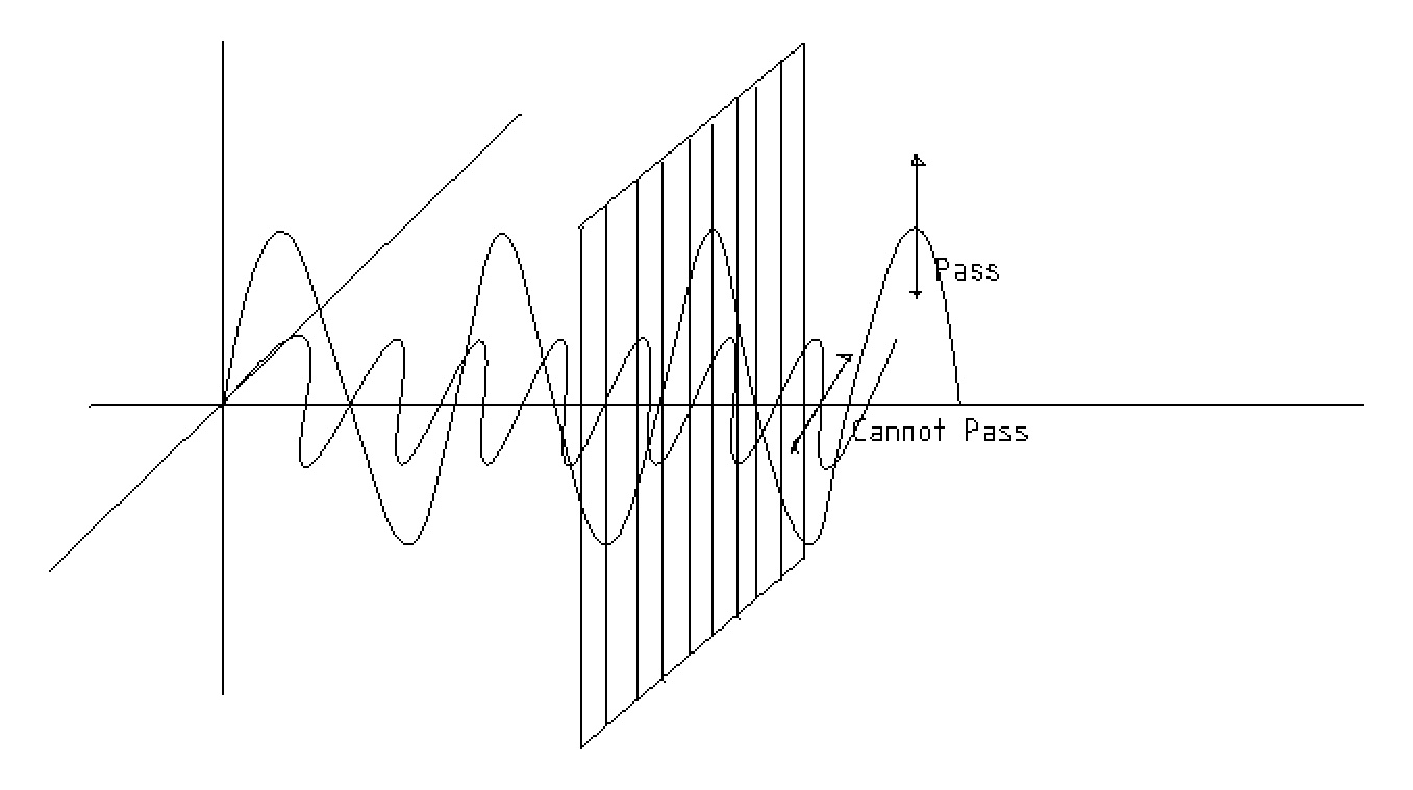
\includegraphics[height=4cm]{wave_charts/pol_dir.eps}
                \end{center}
                \caption{Polarization direction}
                \label{pol_dir}
            \end{figure}

        \paragraph{Intensity after polarization}
            For unpolarized wave with intensity $I_0$, the amplitude of the wave is
            \begin{align}
                & k{A_0}^2 = I_0 \\ 
                & \Rightarrow A_0 = \sqrt{\frac{I_0}{k}}
            \end{align}

            For a polarized wave with the angle between grating and oscillate direction is $\theta$ and intensity $I_0$, the intensity after polarized is 
            \begin{align}
                I_t &= k {A_t}^2 \\
                    &= k (\cos \theta A_0)^2 \\
                    &= (\cos \theta)^2 k {A_0}^2 \\
                    &= (\cos \theta)^2 I_0
            \end{align}

            Thus, for unpolarized wave after polarization, the intensity is 
            \begin{align}
                I &= \int_{0}^{2 \pi} (\cos \theta)^2 \frac{I_0}{2 \pi} \mathrm{d} \theta \\
                  &= \frac{1}{2} I_0
            \end{align} 

    \subsection{Refraction}
        \paragraph{Snell's law}
            As shown in Figure \ref{refre_dia}, a light shoot from refraction index $n_1$ to refraction index $n_2$. The incident angle is $\theta_1$, the refraction angle is $\theta_2$.

            \begin{figure}[H]
                \begin{center}
                    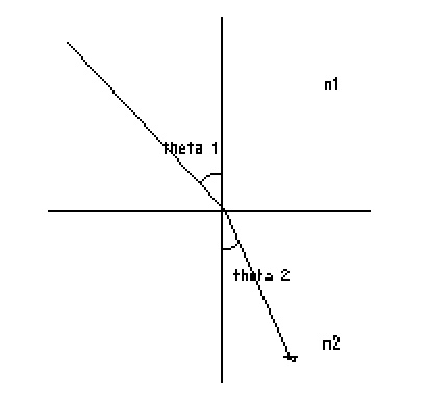
\includegraphics[height=5cm]{wave_charts/refre_dia.eps}
                \end{center}
                \caption{Refrection}
                \label{refre_dia}
            \end{figure}

            Snell'law states that
            \begin{align}
                \sin \theta_1 n_1 = \sin \theta_2 n_2
            \end{align}

            Proof: Pass.

            % TODO
        
    \subsection{Doppler effect}
        Frequency of wave change due moving of observer and radiator.

        \paragraph{Stationary source, approaching viewer}
            In Figure \ref{de_ssav}, the wave have speed $v$ and wave length $\lambda$. The viewer is approaching at speed $v_v$. 
            \begin{figure}[H]
                \begin{center}
                    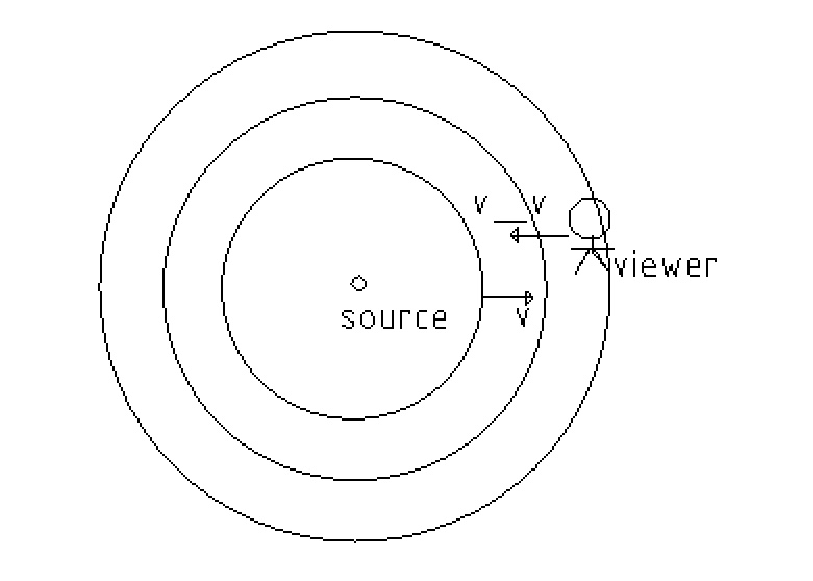
\includegraphics[height=5cm]{wave_charts/dopeff_sta_sou_app_vie.eps}
                \end{center}
                \caption{Stationary source, approaching viewer}
                \label{de_ssav}
            \end{figure}

            The frequency of the wave is $f_0 = \frac{v}{\lambda}$

            The frequency to viewer is
            \begin{align}
                f' &= \frac{v'}{\lambda'} \\
                   &= \frac{v + v_v}{\lambda} \\
                   &= f_0 \frac{v + v_v}{v}
            \end{align}

        \paragraph{Stationary source, leaving viewer}
            Similar to approaching viewer, the frequency to viewer is
            \begin{align}
                f' &= \frac{v - v_v}{\lambda} \\
                   &= f_0 \frac{v - v_v}{v}
            \end{align}

        \paragraph{Approaching source, stationary viewer}
            In Figure \ref{de_assv}, the wave have speed $v$ and wave length $\lambda$. The source is approaching the viewer with speed $v_s$.
            \begin{figure}[H]
                \begin{center}
                    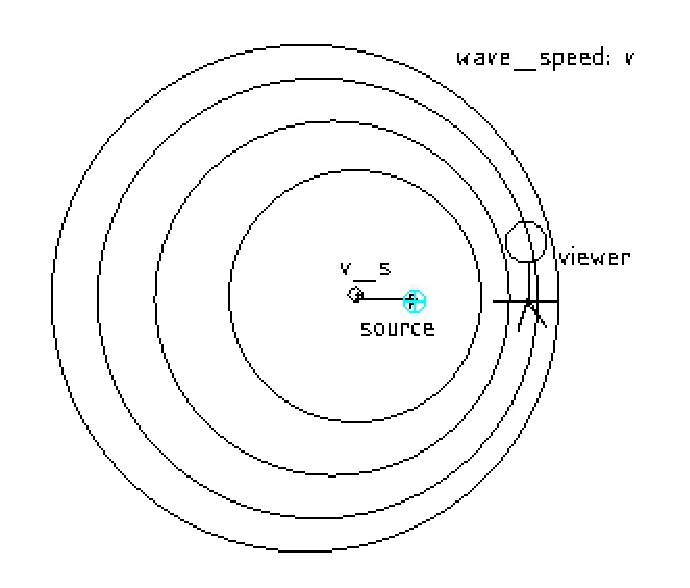
\includegraphics[height=5cm]{wave_charts/dopeff_app_sou_sta_vie.eps}
                \end{center}
                \caption{Approaching source, stationary viewer}
                \label{de_assv}
            \end{figure}

            The wave frequency is $f_0 = \frac{v}{\lambda}$

            The frequency to the viewer is
            \begin{align}
                f' &= \frac{v'}{\lambda'} \\
                   &= \frac{v}{\frac{v - v_s}{f_0}} \\
                   &= f_0 \frac{v}{v - v_s}
            \end{align}

        \paragraph{Leaving source, stationary viewer}
            Samilarly, 
            \begin{align}
                f' = f_0 \frac{v}{v + v_s}
            \end{align}

        \paragraph{Moving source and moving viewer}
            Define the direction from source to viewer as position. The wave frequency is $f_0$ and speed is $v$. The source speed is $v_s$, the viewer speed is $v_v$.

            The frequency observed at viewer is
            \begin{align}
                f' = f_0 \frac{v - v_v}{v + v_s}
            \end{align}

        \paragraph{Doppler effect of EM wave}
            The change in frequency $\Delta f$, with relative motion speed $v$ between viewer and source (approaching is positive), is
            \begin{align}
                \frac{\Delta f}{f_0} &= \frac{\Delta \lambda}{\lambda_0} \\
                                     &\approx \frac{v}{c}
            \end{align}

            Thus, the observed frequency is
            \begin{align}
                f' &= f_0 + \Delta f \\
                   &= f_0 + f_0 \frac{v}{c} \\
                   &= f_0 (1 + \frac{v}{c})
            \end{align}

    \subsection{Wave shock}
        As shown in Figure \ref{wave_shock}, when the speed of the source $v_s$ approach wave speed $v$, and then increase to $v + \tau, \tau \approx 0$, the wave shock. 
        \begin{figure}[H]
            \begin{center}
                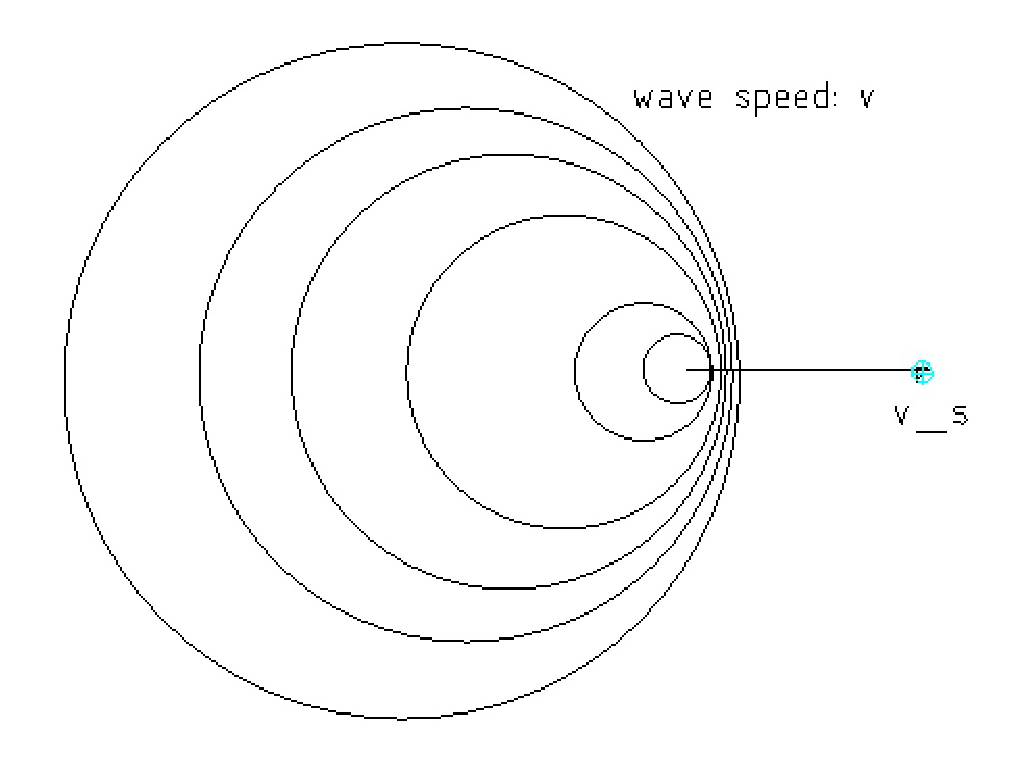
\includegraphics[height=5cm]{wave_charts/wave_shock.eps}
            \end{center}
            \caption{Wave shock}
            \label{wave_shock}
        \end{figure}

        This is the cause of sound boom.

    \subsection{Wave interferance}
        Two wave meet and produce a new wave. 

        \paragraph{Constructive}
            When the wave have same frequency and at the point the wave phase distance is $k \lambda, k \in N$, the point is constructive.

        \paragraph{Destructive}
            At point the wave phase difference is $(k + \frac{1}{2}) \lambda, k \in N$, the point is destructive.

        \paragraph{Double slit interferance}
            As shown in Figure, light with wave length $\lambda$ pass through two slits with distance $d$ and form a interferance partern on screen at distance $L$.
            \begin{figure}[H]
                \begin{center}
                    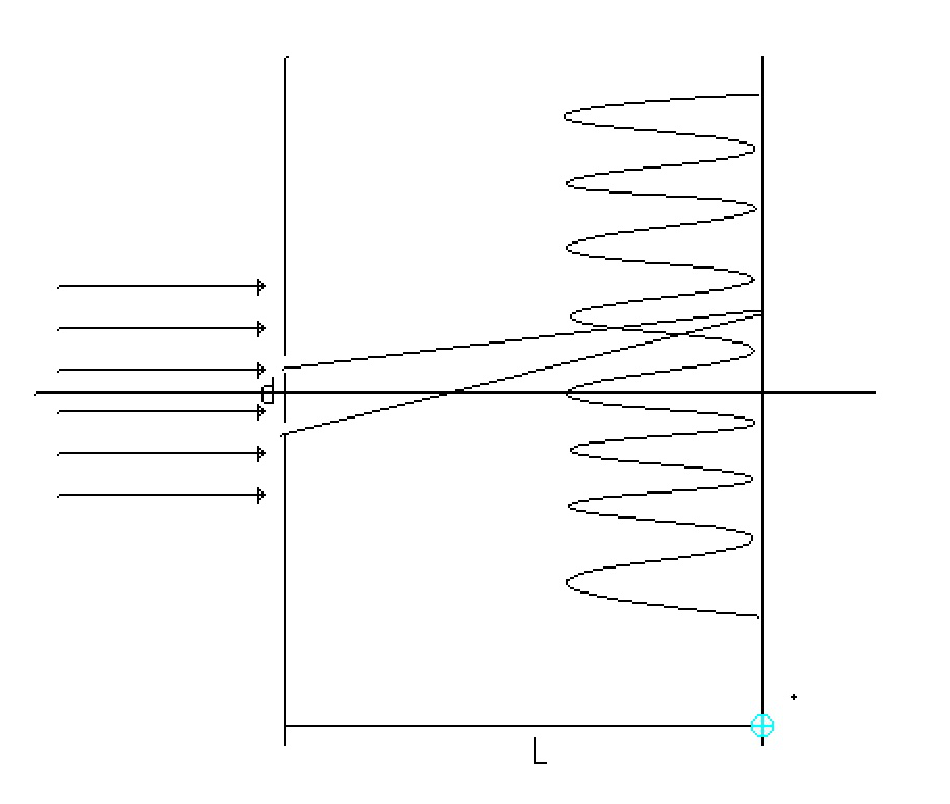
\includegraphics[height=6cm]{wave_charts/doub_slit.eps}
                \end{center}
                \caption{Double slit interferance}
                \label{doub_slit}
            \end{figure}

            The angle of maximas are
            \begin{align}
                & \theta d \approx \sin \theta = n \lambda \\
                & \Rightarrow \theta \approx \sin \theta = \frac{n \lambda}{d}
            \end{align}

            Minimums are 
            \begin{align}
                \theta \approx \sin \theta = \frac{(n + \frac{1}{2}) \lambda}{d}
            \end{align}

        \paragraph{Grating interferance}
            Let the density of grating be $\rho = n / \mathrm{m}$.

            \begin{align}
                d = \frac{1}{\rho}
            \end{align}

            Therefore angle of maximas are
            \begin{align}
                \theta &= \frac{n \lambda}{\frac{1}{\rho}} \\
                       &= n \rho \lambda
            \end{align}

            Minimums are
            \begin{align}
                \theta = (n + \frac{1}{2}) \rho \lambda
            \end{align}

    \subsection{Diffraction}
        Wave spread after passing small slit or hole.

        \paragraph{Single slit diffraction}
            As shown in Figure \ref{sin_slit}, light with wave length $\lambda$ pass through a slit with width $d$ and form a diffraction partern on screen at distance $L$.

            \begin{figure}[H]
                \begin{center}
                    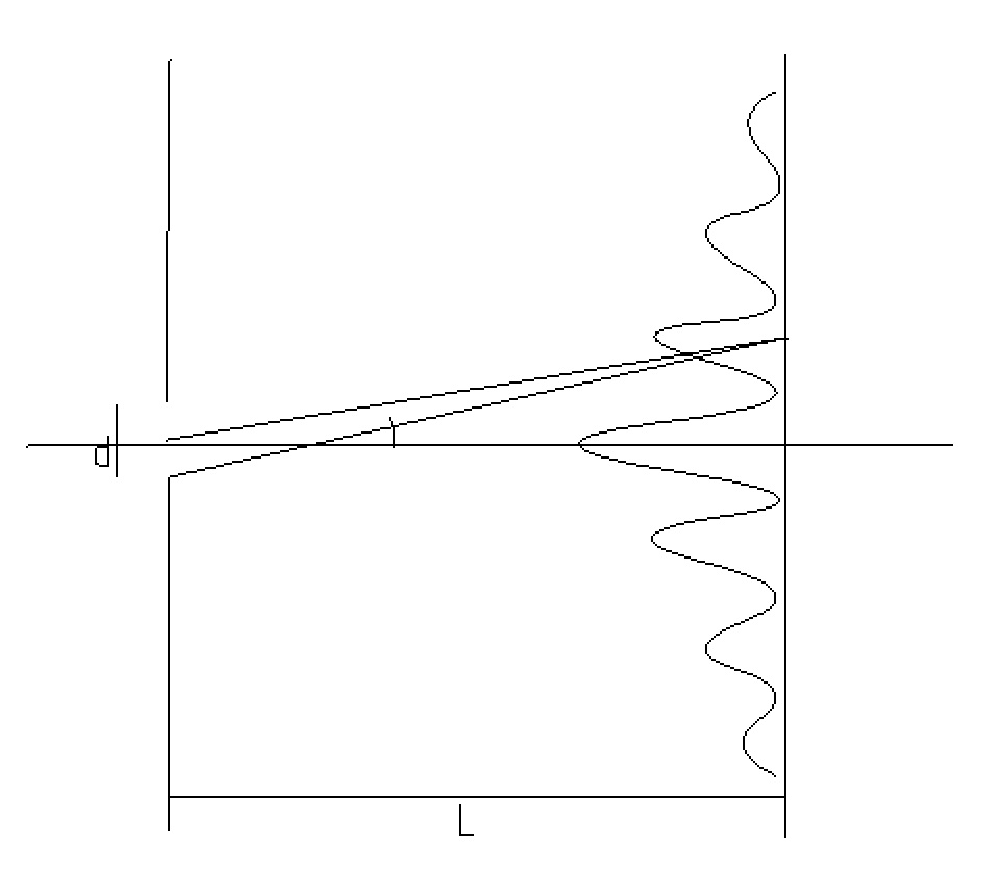
\includegraphics[height=6cm]{wave_charts/sing_slit.eps}
                \end{center}
                \caption{Single slit diffraction}
                \label{sin_slit}
            \end{figure}

            Thus, the angle of maximums are
            \begin{align}
                & \sin \theta \frac{d}{2} = n \lambda, n \in N \\
                & \Rightarrow \theta \approx \sin \theta = \frac{2 n \lambda}{d}
            \end{align}

            Angle of minimums
            \begin{align}
                \theta \approx \sin \theta = \frac{(2n + 1) \lambda}{d}
            \end{align}

            The angular width of central minimum is
            \begin{align}
                \theta = \frac{2 \lambda}{d}
            \end{align}

    \subsection{Anti-reflection coating}
        \paragraph{Half-way loss}
            When wave shoot from low refrection index to high refrection index, the reflected wave have a $\frac{1}{2} \lambda$ phase change from incident wave.

            When shoot from low index to high, no such phase change.

        \paragraph{AR-coating}
            As shown in Figure \ref{ant_ref_coa}, the equations of two reflected wave are $f_1$ and $f_2$. wave speed is $v$, thickness of the plate is $d$.

            \begin{figure}[H]
                \begin{center}
                    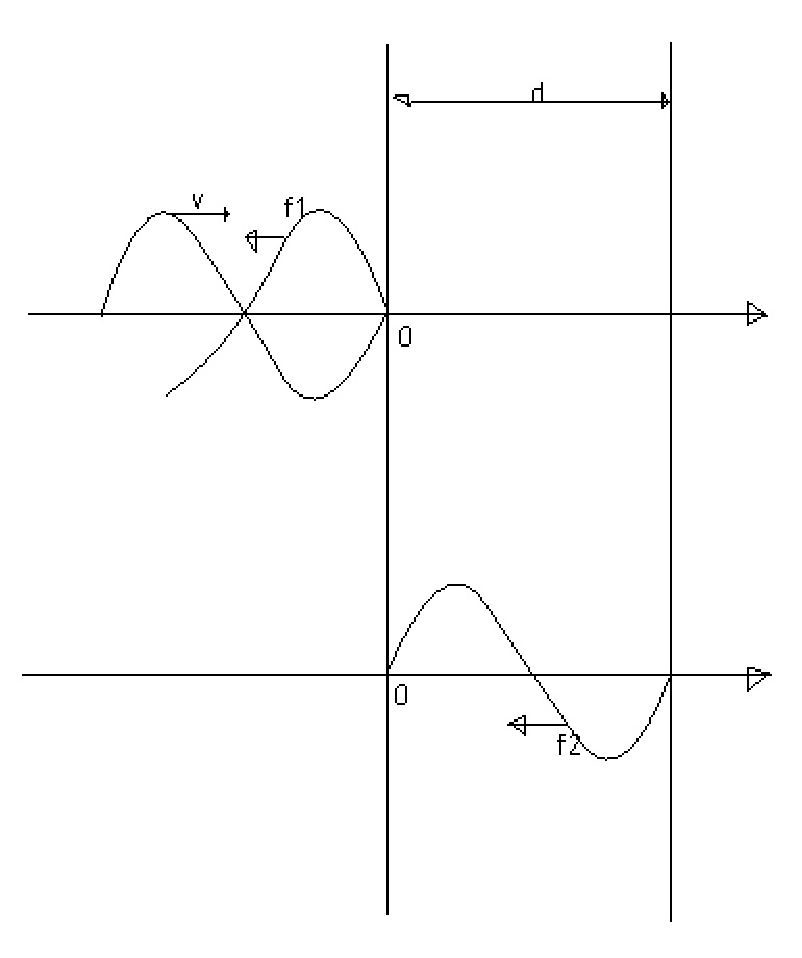
\includegraphics[height=5cm]{wave_charts/ant_ref_coa.eps}
                \end{center}
                \caption{Anti reflection coating}
                \label{ant_ref_coa}
            \end{figure}
            
            The equation of first reflection is 
            \begin{align}
                f_1 = \sin (v t)
            \end{align}

            Equation of second reflection is
            \begin{align}
                f_2 &= - \sin (d - vt + d) \\
                    &= \sin (vt - 2d)
            \end{align}

            % \begin{align}
            %     f_1 + f_2 = \sin(v t) + \sin(v t - 2d)
            % \end{align}

            If constructive, 
            \begin{align}
                & f_1 = f_2 \\
                & \Rightarrow 2 d = n \lambda
            \end{align}

            If destructive,
            \begin{align}
                & f_1 + f_2 = 0 \\
                & \Rightarrow 2d = (\frac{1}{2} + n) \lambda
            \end{align}

            Thus, for anti reflection coating, the coating thickness is
            \begin{align}
                d = (\frac{1}{4} + \frac{n}{2}) \lambda
            \end{align}

            NOTE: The $\lambda$ is the wave length inside the coating. Need to consider refrection index.
    
    \subsection{Resolution}
        \paragraph{Circular hole interferance}
            The angular width of the interferance partern of circular hole is 1.22 times the single slit one.

            First minimum:
            \begin{align}
                \theta = 1.22 \frac{\lambda}{d}
            \end{align}

        \paragraph{Resolution}
            Figure \ref{just_resol} show two light (object) with wave length $\lambda_1$ and $\lambda_2$ pass through the circular slit and just resolve.

            \begin{figure}[H]
                \begin{center}
                    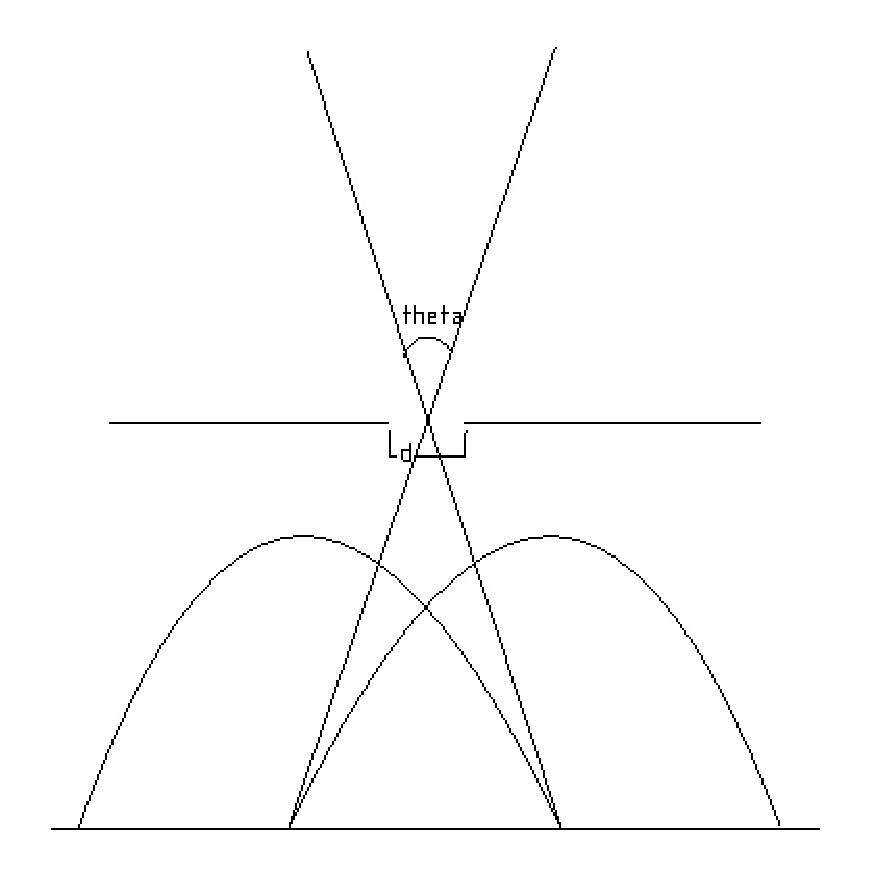
\includegraphics[height=6cm]{wave_charts/resol.eps}
                \end{center}
                \caption{Just resolve}
                \label{just_resol}
            \end{figure}

            Let the minimum angle of seperation of two objects be $theta$ to be resolve. 
            \begin{align}
                & 1.22 \frac{\bar{\lambda}}{d} = \theta \\
                & \Rightarrow \theta = 1.22 \frac{\lambda_1 + \lambda_2}{2 d}
            \end{align}

    \subsection{Standing wave}
        \paragraph{How to form}
            A wave met and interferance with its reflected wave and form a new wave. The new wave is standing wave.

        \paragraph{Period}
            The standing wave have same period.

        \paragraph{Standing wave in pip}
            If both end closed, shown in Figure \ref{stan_2endpip}.
            \begin{figure}[H]
                \begin{center}
                    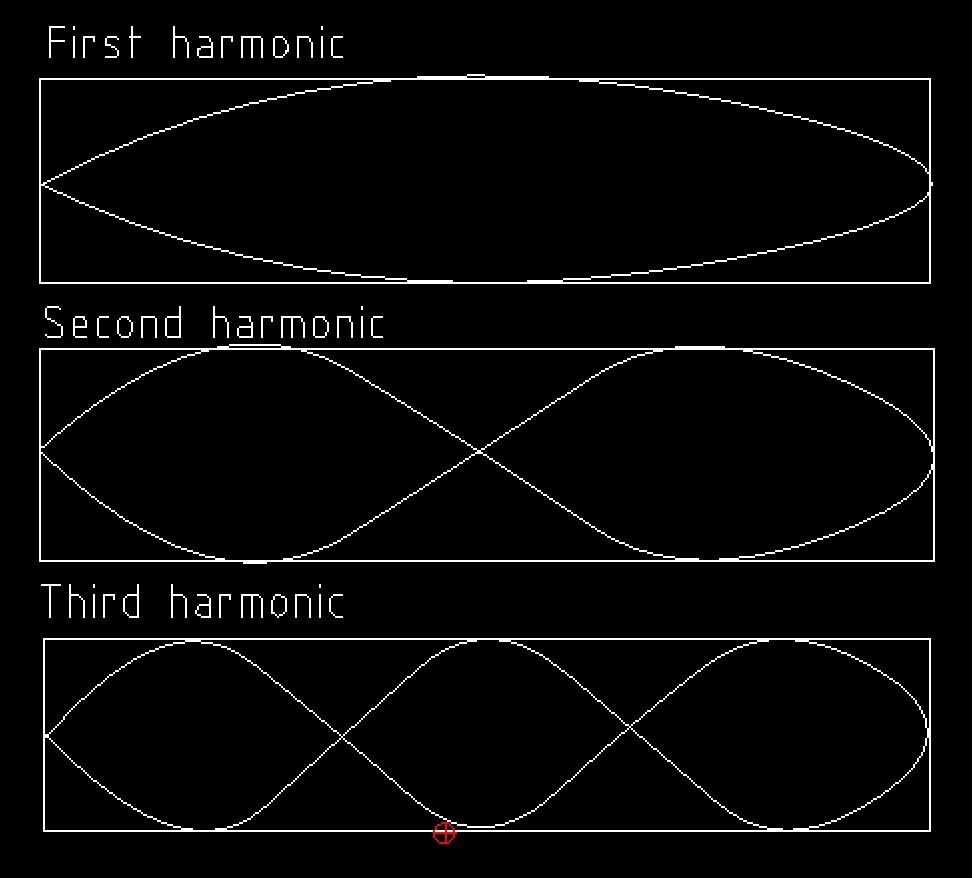
\includegraphics[height=5cm]{wave_charts/stan_wav_2endpipe.eps}
                \end{center}
                \caption{Harmonics in a pip with both end closed}
                \label{stan_2endpip}
            \end{figure}

            The $n^{\mathrm{th}}$ harmonic have $\frac{n}{2}$'s period. Thus,
            \begin{align}
                L &= \frac{n}{2} \lambda \\
                \Rightarrow \lambda &= \frac{2}{n} L, n \in Z^+
            \end{align}

            If one end closed and one end open, shown in Figure \ref{stan_1endpip}.
            \begin{figure}[H]
                \begin{center}
                    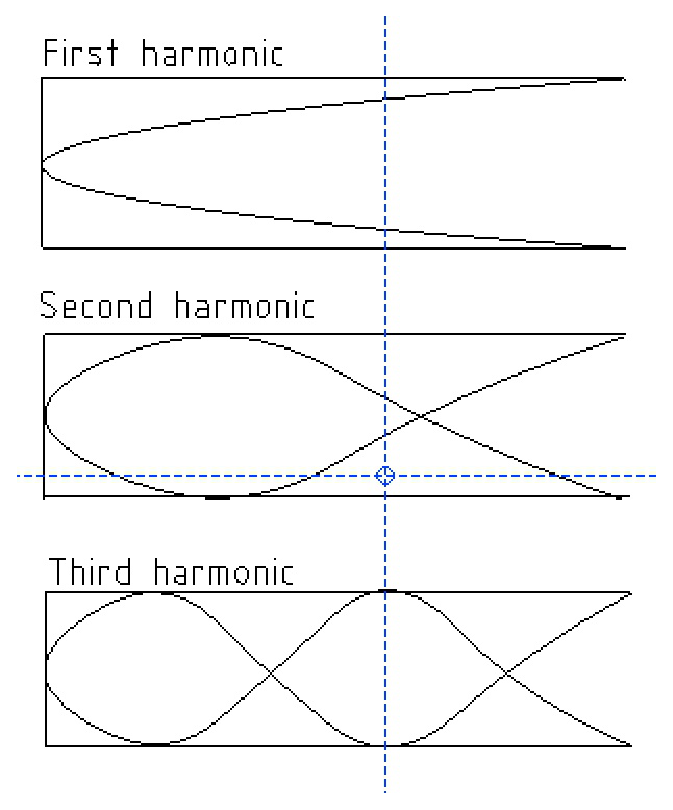
\includegraphics[height=5cm]{wave_charts/stan_wav_1endpipe.eps}
                \end{center}
                \caption{Harmonics in a pip with one end closed and one end open}
                \label{stan_1endpip}
            \end{figure}

            The $n^{\mathrm{th}}$ harmonic have $\frac{1}{2} n - \frac{1}{4}$'s period. Thus,
            \begin{align}
                L &= (\frac{n}{2} - \frac{1}{4}) \lambda \\
                \Rightarrow \lambda &= \frac{4 L}{2 n - 1}, n \in Z^+
            \end{align}

            If both end open, shown in Figure \ref{stan_0endpip}.
            \begin{figure}[H]
                \begin{center}
                    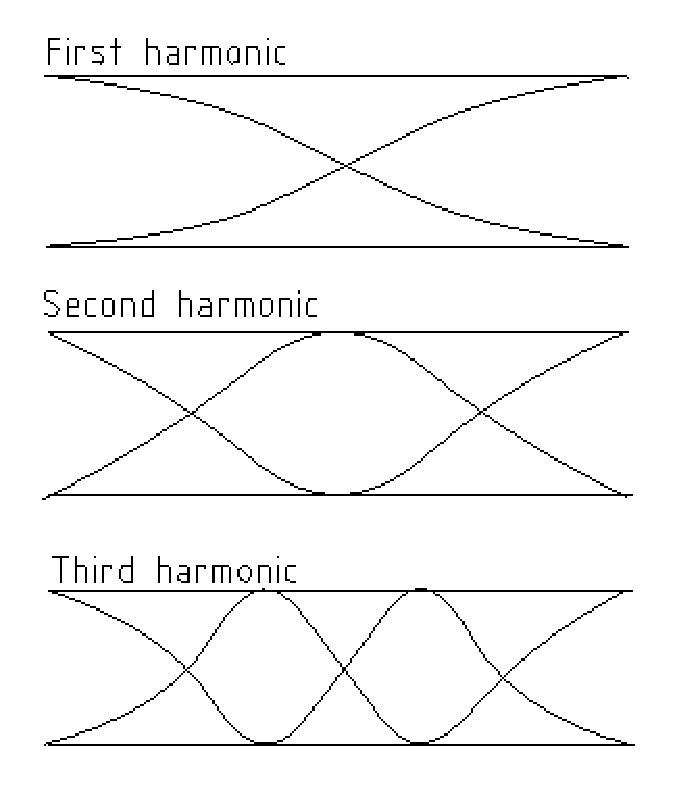
\includegraphics[height=5cm]{wave_charts/stan_wav_0endpipe.eps}
                \end{center}
                \caption{Harmonics in a pip with both end open}
                \label{stan_0endpip}
            \end{figure}

            The $n^{\mathrm{th}}$ harmonic have $\frac{n}{2}$'s period. Thus
            \begin{align}
                L &= \frac{n}{2} \lambda \\
                \Rightarrow \lambda &= \frac{2 L}{n}
            \end{align}

        \paragraph{Standing wave in string}
            Same model as two-end-closed pipe.